\chapter{Ten micrometres: the results}\label{ch:ten_results}

In every comparison of this chapter, \textbf{MAGIC-UNet} means run B (0.7\um\ pixels, 44.8\um\ tile) with the
data-consistency step of Chapter~\ref{ch:consistency} at the height the network itself estimates. Run A appears only
where the tile size is the subject.

\section{On simulation}

\begin{center}
\begin{tabular}{lcc}
\toprule
Simulation, 10\um\ to 0.5\um & Error & Layouts \\
\midrule
MAGIC-UNet & \textbf{15.8\%} & 50 \\
MAGIC-UNet, on the 20 layouts below & \textbf{14.7\%} & 20 \\
FISTA, 3{,}000 iterations & 48.8\% & 20 \\
CSC-LISTA, with its 3\um\ settings & 91.8\% & 20 \\
FISTA-Net & still training & \\
\bottomrule
\end{tabular}
\end{center}

MAGIC-UNet is better than FISTA on all 20 layouts. FISTA is told the standoff. MAGIC-UNet is not.

\begin{figure}[H]
\centering
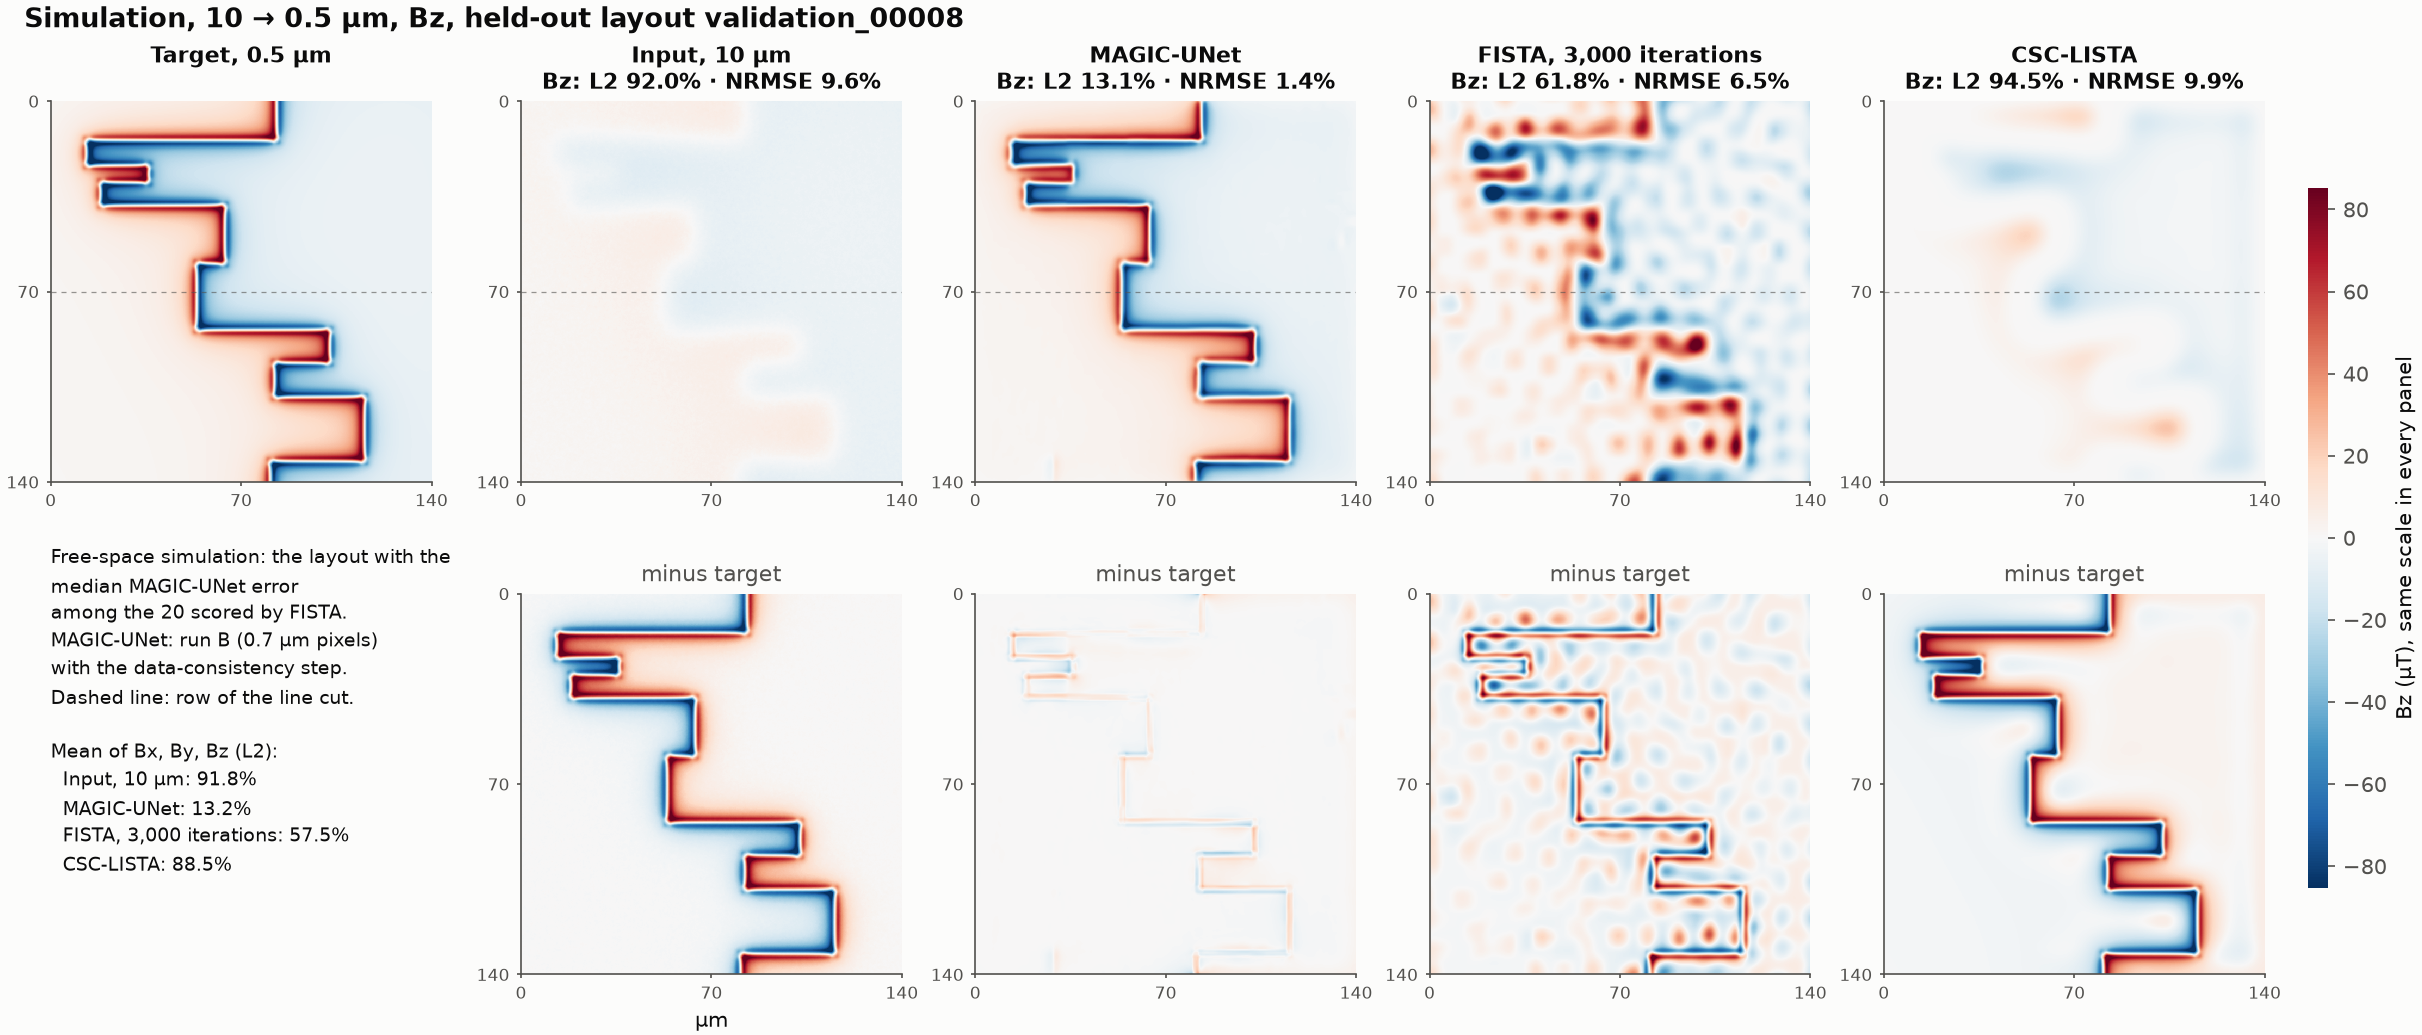
\includegraphics[width=\textwidth]{hs_sim_median_maps}
\caption{A held-out simulated layout, chosen by a rule: the one with the median MAGIC-UNet error among the 20 layouts.
Every panel uses the same colour scale, so the nearly blank second panel is the true size of the measured field. Bottom
row: output minus target.}
\label{fig:hs_sim}
\end{figure}

Look at what each method does in Figure~\ref{fig:hs_sim}. The measurement holds a faint, smooth shadow of the wire.
FISTA finds where the wire runs, but it can only rebuild what its dictionary and the measurement support, and the wire
comes out as a string of blobs. MAGIC-UNet draws a wire: a continuous path of constant width. It has learned that
currents come in wires, and it uses the shadow only to decide where the wire goes.

\begin{figure}[H]
\centering
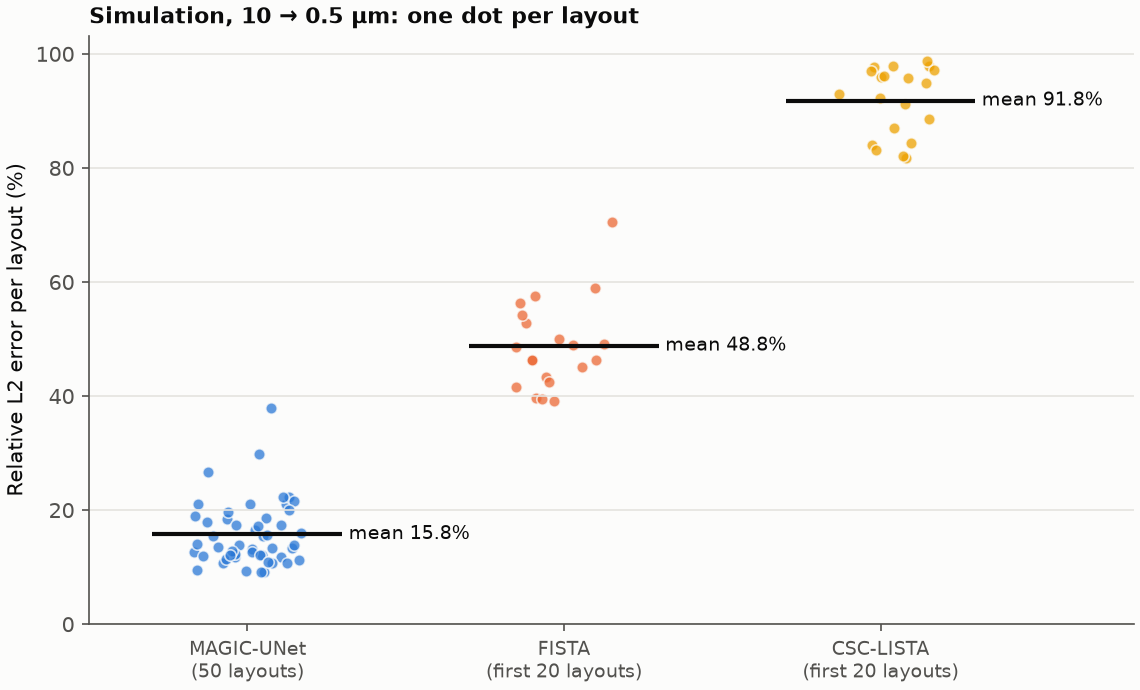
\includegraphics[width=0.7\textwidth]{hs_per_layout_10um}
\caption{One dot per layout at 10\um\ to 0.5\um.}
\label{fig:hs_dots}
\end{figure}

\begin{careful}[What 15.8\% is, and is not]
The test layouts are new, but they come from the same simulator as the training layouts: the same three families of
layout, wire widths of 1.6--3.2\um\ and one current of 600\,\textmu A. At 10\um\ nearly all of the 0.5\um\ field is prior
band (Chapter~\ref{ch:limits}), so nearly all of the output comes from what the network learned wires look like. That is
what a learned source prior is for. It is also its limit: nothing here says the number holds for other wire shapes or
several currents. The review's second risk, ``the prior has memorised the simulator'', is not answered by this test.
\end{careful}

\section{The tile size is what makes it work}

\begin{center}
\begin{tabular}{llcc}
\toprule
Model & Tile & Trained on & Simulation, 10\um\ to 0.5\um \\
\midrule
Run B & 44.8\um & $10\pm2$\um & \textbf{15.8\%} \\
Run A & 12.8\um & $10\pm2$\um & 58.2\% \\
Run 3 & 12.8\um & 1--10\um & 55.4\% \\
Run 2 & 12.8\um & $3\pm0.6$\um & 90.8\% \\
\bottomrule
\end{tabular}
\end{center}

Same network, same layouts, same recipe. With the small tile MAGIC-UNet is \emph{worse} than FISTA. With the large tile
it is three times better. Run B beats run A on all 50 layouts. The measurement of Chapter~\ref{ch:ten} had predicted the
direction before a single epoch was trained.

\begin{figure}[H]
\centering
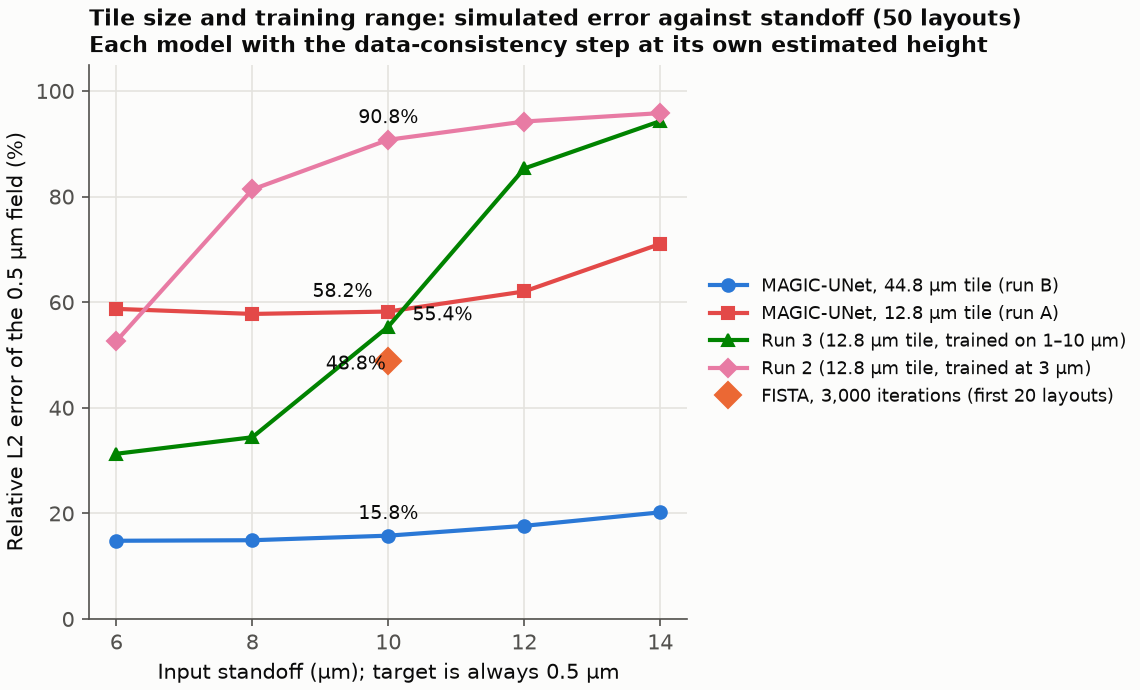
\includegraphics[width=0.85\textwidth]{hs_error_vs_standoff}
\caption{The same 50 layouts at input standoffs from 6 to 14\um. One run B model covers the whole range (14.8--20.2\%)
without being told the height.}
\label{fig:hs_standoff}
\end{figure}

\section{The height read-out and the correction at 10\um}

\begin{figure}[H]
\centering
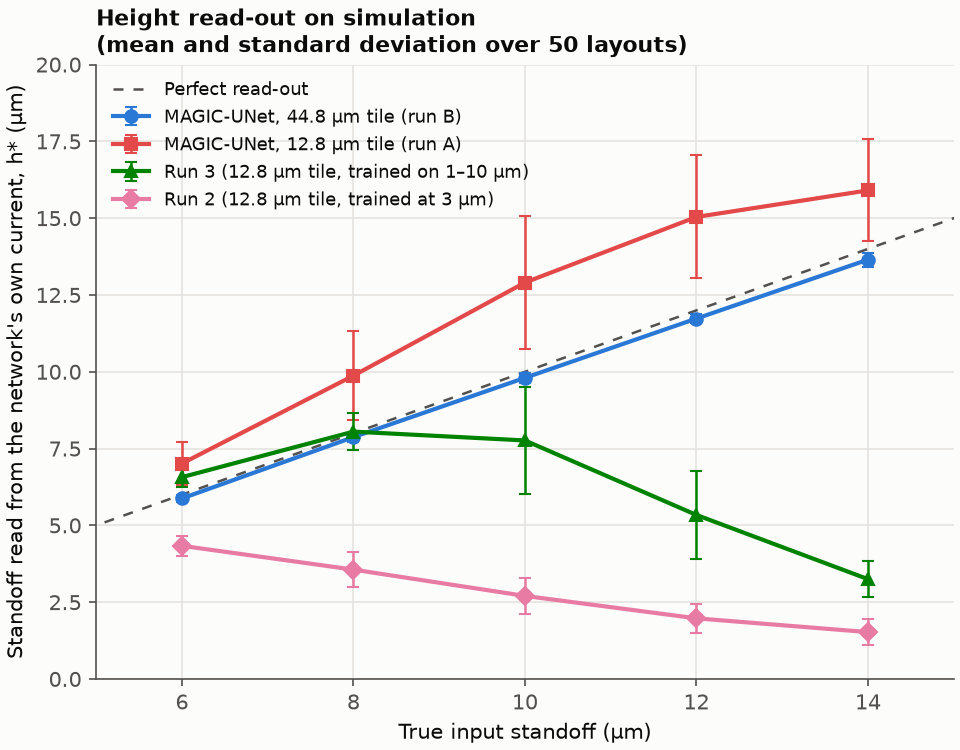
\includegraphics[width=0.6\textwidth]{hs_height_readout}
\caption{Standoff read from each network's own current (Chapter~\ref{ch:height}) against the true standoff.}
\label{fig:hs_height}
\end{figure}

Run B reads 9.80\um\ at a true 10\um, and is within 0.14--0.39\um\ from 6 to 14\um. Run A reads 12.9\um. This is
Chapter~\ref{ch:height} again: the read-out is as good as the current it is read from.

\begin{center}
\begin{tabular}{lcccc}
\toprule
 & Raw & Corrected, true height & Corrected, $h^\ast$ & Best $\mu$ at 10\um \\
\midrule
Run B & 16.3\% & 15.8\% & 15.8\% & 0.178 \\
Run A & 54.8\% & 50.8\% & 58.2\% & 0.0032 \\
\bottomrule
\end{tabular}
\end{center}

Two things to learn from this table.
\begin{itemize}
\item \textbf{For run B the correction hardly matters.} The selection picked a large $\mu$, which means ``leave the network
alone''. Remember the dial $w$ of Chapter~\ref{ch:consistency}: at 10\um\ the measurement only reaches the lowest
frequencies (Figure~\ref{fig:late_dc}, right), and there run B already agrees with it.
\item \textbf{For run A the correction hurts.} At the true height it would help. But run A's height is 3\um\ too high, and a
correction built on a wrong height amplifies in the wrong place. A data-consistency step is only as good as the
height it is given.
\end{itemize}

\section{The FISTA baseline at 10\um}

Everything about FISTA was chosen again on simulated data at 10\um.
\begin{itemize}
\item \textbf{Padding.} The blur is much wider now, so more zero padding might be needed. Tested at 128, 256, 384 and 512
pixels: 63.2, 63.6, 63.9 and 64.0\%. More padding does not help, so 128 stays.
\item \textbf{Penalty.} The best $\lambda$ is thirty to a hundred times smaller than at 3\um.
\item \textbf{Depth.} From the curve of Chapter~\ref{ch:fista_depth}, recorded every 25 iterations.
\end{itemize}

\begin{figure}[H]
\centering
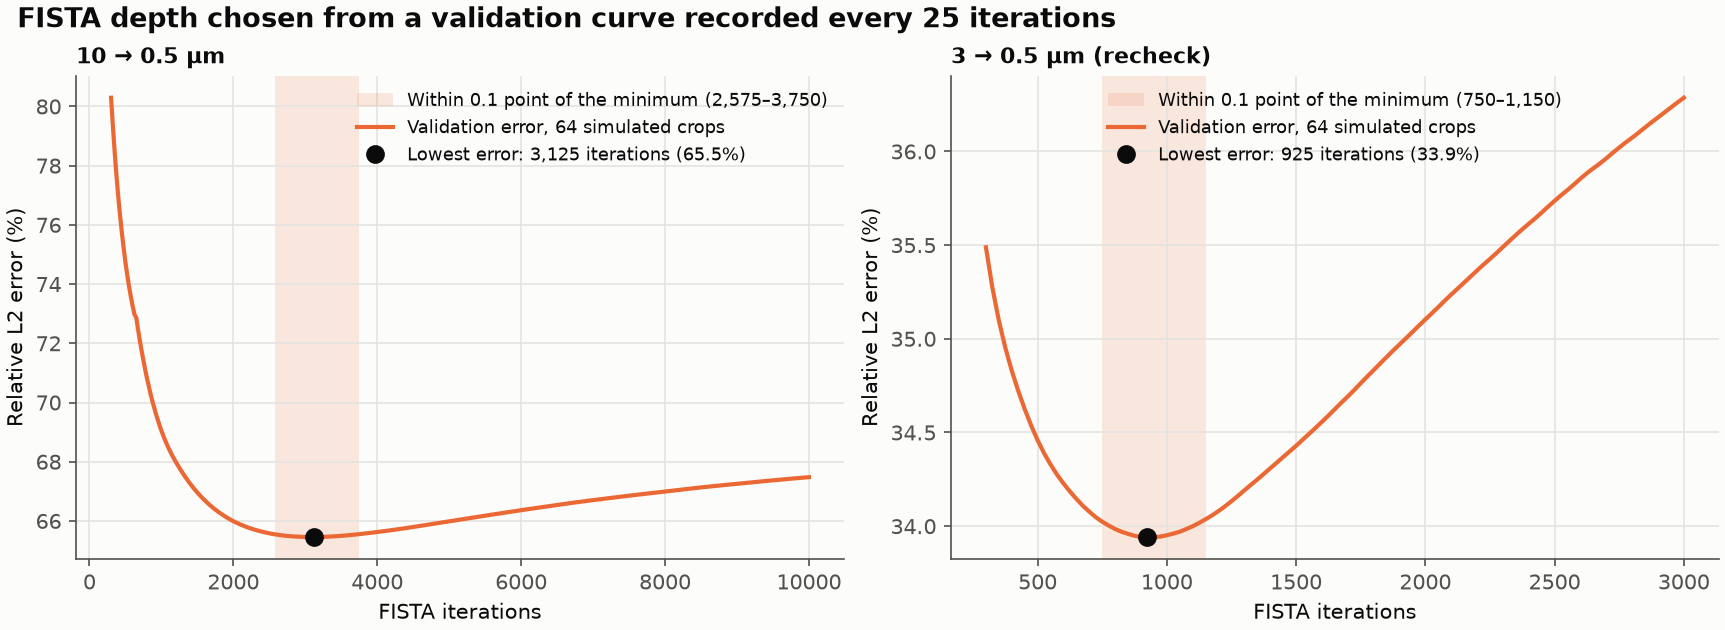
\includegraphics[width=\textwidth]{hs_fista_depth_curves}
\caption{FISTA's error on 64 simulated validation crops against the number of iterations. The dot marks the lowest
error; the band marks every depth within 0.1 points of it.}
\label{fig:hs_fista}
\end{figure}

The first curve ended at 3{,}000 iterations, which was then its lowest point. So the minimum might lie beyond. It was
extended to 10{,}000. The minimum is at \textbf{3{,}125} iterations: 65.46\%, only 0.004 points below the value at
3{,}000, and the curve rises slowly afterwards (67.5\% at 10{,}000). The rule written beforehand asked for a gain of
half a point before re-scoring, so FISTA at 3{,}000 stays the baseline. It is now known to sit at the minimum.

\begin{keyidea}[925 at 3\um, 3{,}125 at 10\um]
FISTA needs more than three times as many iterations at 10\um. The reason is in the gradient step. The step size is
set by the \emph{strongest} frequency the blur lets through. A frequency that the blur weakens by a factor $H$ is then
corrected $H^2$ times more slowly. At 10\um\ the useful frequencies are weakened far more, so they need far more steps.
\end{keyidea}

(The 64-crop curve reads 65\% and the full-image score is 48.8\%. A 51\um\ crop loses the surrounding field that a full
140\um\ image keeps. The full-image number is the one compared with MAGIC-UNet.)

\section{On COMSOL}

\begin{center}
\begin{tabular}{lccc}
\toprule
COMSOL, 10\um\ to 0.5\um & 15 pairs & C1 family & \code{IC_4um} \\
\midrule
FISTA, 3{,}000 iterations & \textbf{54.3\%} & \textbf{50.2\%} & 71.0\% \\
MAGIC-UNet & 59.3\% & 59.6\% & \textbf{58.3\%} \\
CSC-LISTA, with its 3\um\ settings & 98.1\% & 99.6\% & 92.4\% \\
FISTA-Net & \multicolumn{3}{c}{still training} \\
\bottomrule
\end{tabular}
\end{center}

On COMSOL the order flips. FISTA is ahead on the mean and on the C1-family coils. MAGIC-UNet is ahead on
\code{IC_4um}.

\begin{figure}[H]
\centering
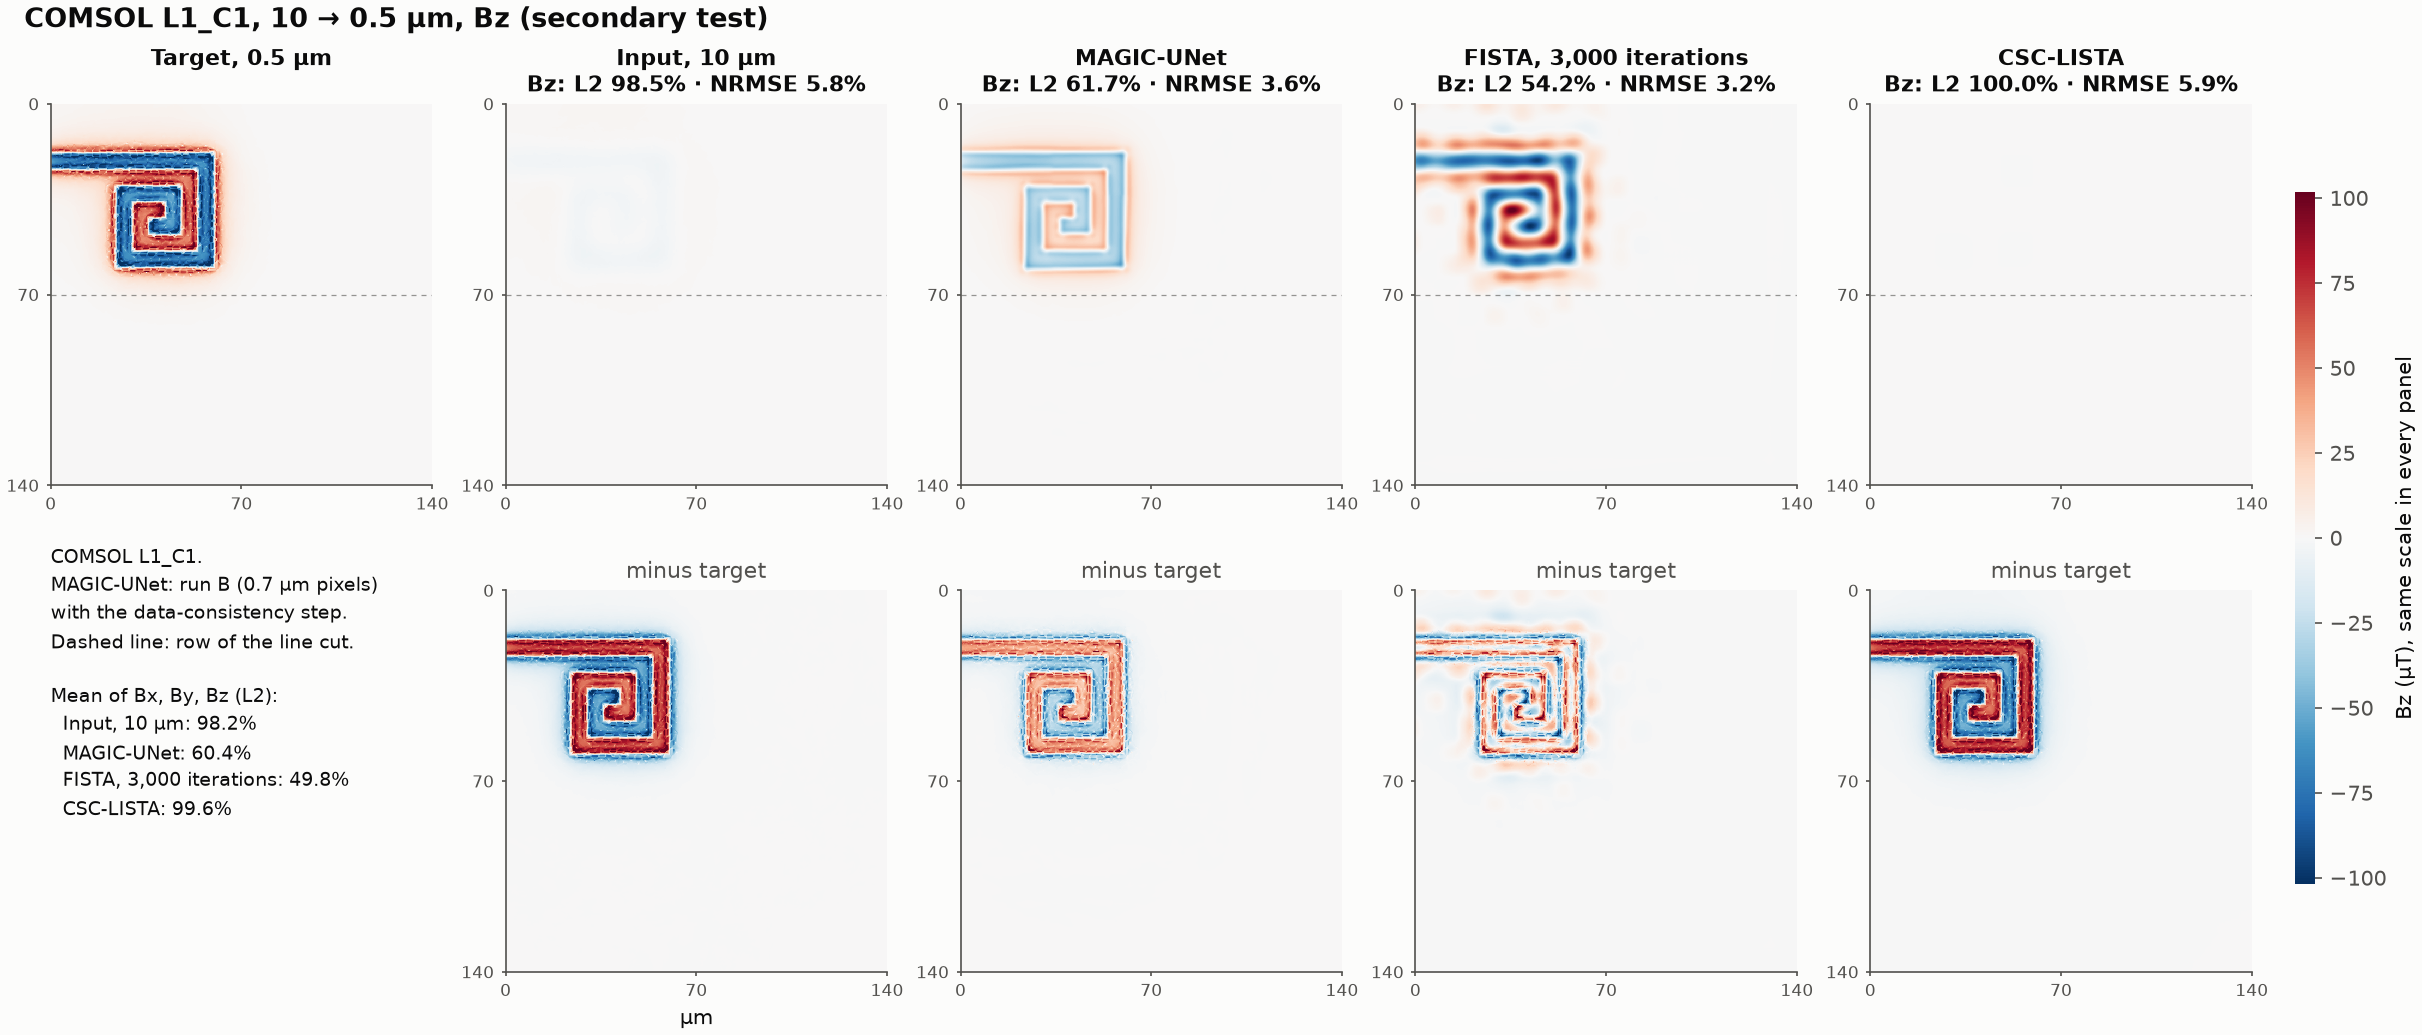
\includegraphics[width=\textwidth]{hs_comsol_L1_C1_maps}
\caption{COMSOL \code{L1_C1}, 10\um\ to 0.5\um. MAGIC-UNet draws the coil in the right place, but too faint.}
\label{fig:hs_comsol}
\end{figure}

\section{Shape and strength, measured separately}

Figure~\ref{fig:hs_comsol} suggests that MAGIC-UNet has the right picture at the wrong brightness. One relative error
cannot tell those apart, so two more numbers are computed:

\begin{code*}{k0_check.py}
        out[f'amp_{c}'] = float(dot[i] / tt[i])
        out[f'cos_{c}'] = float(dot[i] / np.sqrt(pp[i] * tt[i]))
\end{code*}

\code{dot} is the sum of output times target, \code{tt} of target squared, \code{pp} of output squared.
\begin{itemize}
\item \textbf{Amplitude} (\code{amp}): how strong the output is along the target. 1 means the right strength.
\item \textbf{Cosine} (\code{cos}): how alike the two patterns are, whatever their strength. 1 means the same shape.
\end{itemize}

\begin{center}
\begin{tabular}{lccc}
\toprule
COMSOL, C1 family, 10\um\ to 0.5\um & Error & Amplitude & Cosine \\
\midrule
MAGIC-UNet & 59.6\% & 0.42 & 0.95 \\
FISTA, 3{,}000 iterations & 50.2\% & 0.66 & 0.87 \\
\bottomrule
\end{tabular}
\end{center}

MAGIC-UNet has the better shape and less than half the strength. Its COMSOL error is mostly amplitude.

\section{Testing the suspect}

Chapter~\ref{ch:comsol} gives a suspect. COMSOL's field decays faster than physics allows, so its 10\um\ field is weaker
than anything the network was trained on. A weaker field looks, to the network, like a weaker current.

This can be tested without COMSOL. The simulator has the switch of Chapter~\ref{ch:comsol}. Render the same 50 test
layouts again with COMSOL's extra decay in the 10\um\ input, and change nothing else:

\begin{code*}{k0_check.py}
        settings = dict(sim.settings, z_input=Z_IN, z_target=Z_TG, decay_k0=float(k0))
\end{code*}

The reference plane of the switch is 0.5\um, so the target is unchanged; only the input gets weaker. Nothing is
retrained. The rule for reading the result was written first (amendment A5): at the fitted $k_0=0.10$, an error of 45\%
or more means the decay explains most of the gap, 25\% or less means it does not, and in between it explains part.

\begin{center}
\begin{tabular}{lcccc}
\toprule
Extra decay $k_0$ (rad/\um) & MAGIC-UNet error & Amplitude & Cosine & Estimated height \\
\midrule
0 (free space) & 15.8\% & 0.98 & 0.99 & 9.80\um \\
0.05 & 20.7\% & 0.83 & 0.99 & 9.48\um \\
\textbf{0.10 (fitted to COMSOL)} & \textbf{42.0\%} & 0.59 & 0.99 & 8.93\um \\
0.15 & 61.1\% & 0.39 & 0.98 & 8.36\um \\
\midrule
COMSOL, C1 family & 59.6\% & 0.42 & 0.95 & 8.3--8.5\um \\
\bottomrule
\end{tabular}
\end{center}

With no extra decay the check reproduces the saved scores exactly. FISTA, on the 5 layouts it was run on, moves from
47.9\% to 49.4\%.

\begin{figure}[H]
\centering
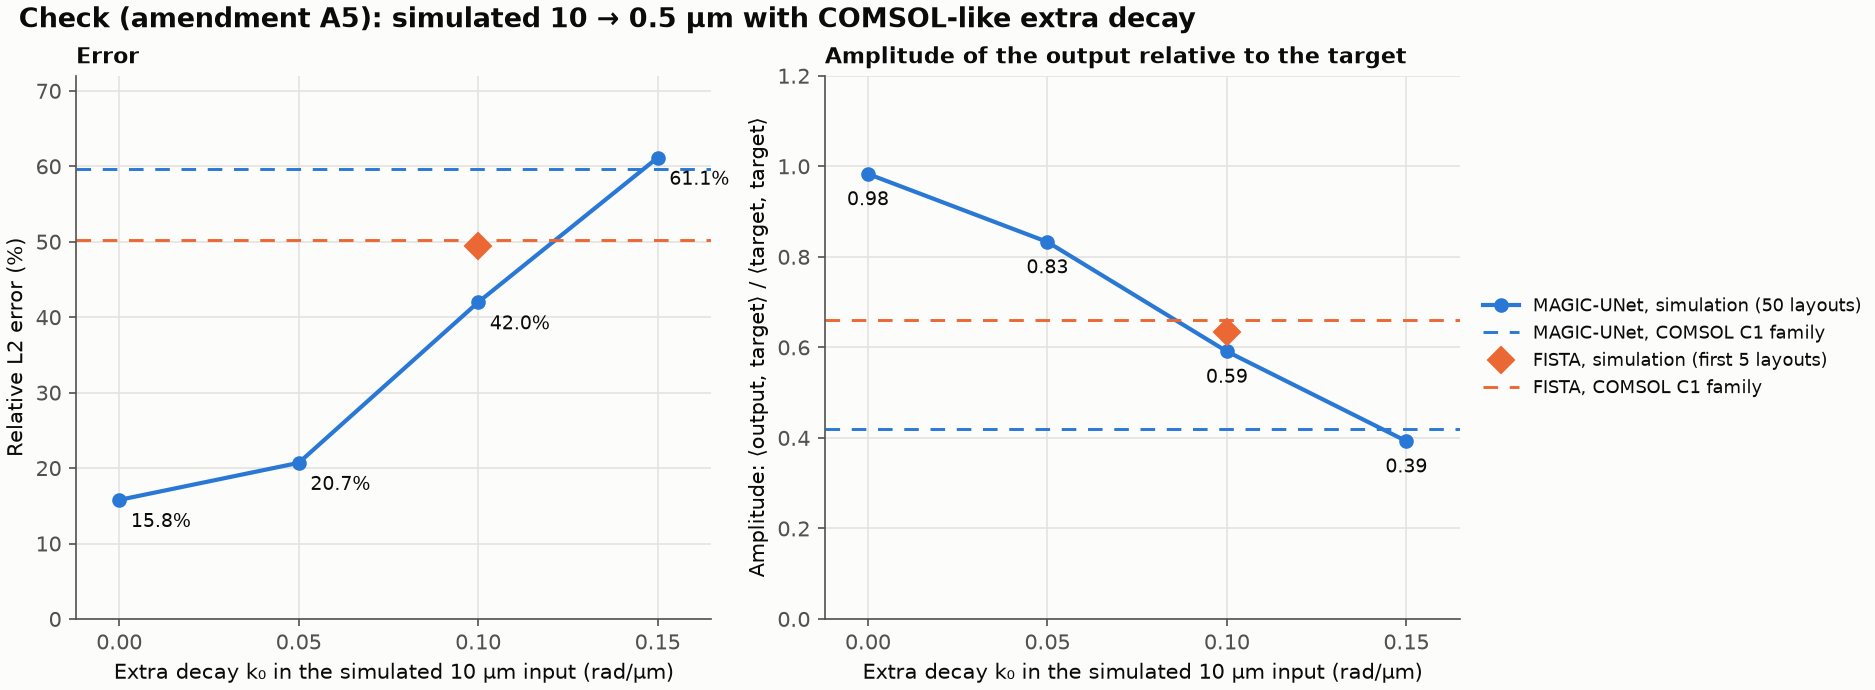
\includegraphics[width=\textwidth]{hs_k0_check}
\caption{MAGIC-UNet and FISTA on simulation as COMSOL-like extra decay is added. Dashed lines: each method's value on
the COMSOL C1-family coils.}
\label{fig:hs_k0}
\end{figure}

\begin{keyidea}[What the check shows]
\begin{itemize}
\item \textbf{The extra decay explains part of the gap:} about 26 of the 44 points between 15.8\% and 59.6\%, at the fitted
$k_0$. The other 18 are not explained.
\item \textbf{It does not flip the order.} At $k_0=0.10$ MAGIC-UNet is still ahead of FISTA (43.4\% against 49.4\% on the
same 5 layouts).
\item \textbf{The error it causes is of the same kind as on COMSOL:} right pattern, weak amplitude, low height estimate.
\item \textbf{MAGIC-UNet is sensitive to the physics of the measurement, and FISTA is not.} FISTA moves by 1.5 points,
MAGIC-UNet by 26. A learned prior inherits the physics of its training data.
\end{itemize}
\end{keyidea}

This also settles the loose end of Chapter~\ref{ch:height}. Run 3 read COMSOL heights too \emph{low} at large standoffs,
and on simulation too high. The last column shows why: extra decay makes a network read a smaller height.

\begin{careful}[What the check does not show]
At $k_0=0.15$ all three numbers land close to their COMSOL values, and 0.15 is inside the range estimated for COMSOL
(0.07--0.17). But it is not the fitted value, and FISTA was not run there. Treat it as a hint. The check also leaves
out COMSOL's walls, its mesh noise and the coil shapes themselves.
\end{careful}

\section{CSC-LISTA does not survive the move to 10\um}

You asked for the other learned methods at 10\um\ too. They had only ever been trained for 3\um. So they were trained
again with the same frozen code and the same settings, and only two things changed: the blur in the operator, and the
height at which the training layouts are rendered. For CSC-LISTA (strict, 64 layers, 33.8\% at 3\um):

\begin{center}
\begin{tabular}{lcccc}
\toprule
Training step & 0 (untrained) & 100 & 500 & 1{,}000 \\
\midrule
Validation error, 64 crops & \textbf{89.8\%} & 102.7\% & 119.9\% & 120.9\% \\
\bottomrule
\end{tabular}
\end{center}

Its best checkpoint is the one \emph{before any training}. Training made it worse. The final scores, 91.8\% on simulation
and 98.1\% on COMSOL, are close to doing nothing: the measured input itself is at about 92--98\%.

Two reasons were written down before the run. Recall from Chapter~\ref{ch:csc_lista} that each layer has a learned
filter $W$, started from the blurred dictionary and cut to a fixed size:

\begin{code*}{csc_lista.py}
        # ISTA start: w = d / L, truncated to the filter support.
\end{code*}
\begin{code*}{csc_lista.py}
            rows.append(full[..., :width, :width] * step)
\end{code*}

\code{width} is 155 pixels, 15.5\um. At 3\um\ the blur is about 4\um\ wide and fits easily. At 10\um\ the blur is as
wide as the filter itself, so cutting it off throws away much of what it should contain, and the layers start from the
wrong operator. The second reason: 64 layers are 64 iterations, and the previous section showed that plain FISTA on the
same dictionary needs about 3{,}000 here.

\begin{careful}
This is a statement about CSC-LISTA \emph{as configured for 3\um}, with only the standoff changed, as you asked. Wider
filters or more layers were not tried, and the run already used 40 of the GPU's 49\,GB. FISTA-Net has only 7 layers; it
is still training and may fail in the same way.
\end{careful}

\section{What can be claimed}

\begin{keyidea}[The fair summary at 10\um]
On free-space simulated data, MAGIC-UNet with a tile matched to the blur reconstructs the 0.5\um\ field from 10\um\ with
15.8\% error, three times better than a converged FISTA, without being told the standoff, and one model covers
6--14\um. On COMSOL at 10\um\ it does \textbf{not} beat FISTA. Part of that is COMSOL's own physics; the rest is open.
\end{keyidea}

\begin{defend}[If your professor asks: 15\% at 10\um\ sounds too good. Is it real?]
It is real on its test set, and the test set is honest about what it is: new layouts from the simulator that made the
training data. The export for the figures reproduced every saved score. It shows that a source prior can recover what
the measurement lost, when the sources look like the training sources. It does not show that the number holds for a
device with other wire shapes or currents.
\end{defend}

\begin{defend}[If your professor asks: then why believe the simulation and not COMSOL?]
Because of Chapter~\ref{ch:comsol}. Above about 4\um\ COMSOL's field breaks Amp\`ere's law in empty air by 27--52\%, and
our simulator matches exact Biot--Savart to under 1\%. But do not hide the COMSOL result. Report both, and report the
check that explains part of the difference.
\end{defend}

\begin{defend}[If your professor asks: what is the weakness of the learned method?]
It depends on the physics it was trained on. A field that decays a little faster than its training fields costs it 26
points, where FISTA loses 1.5. The good news is that the failure announces itself: the output keeps its pattern but
loses strength, and the height read-out drops.
\end{defend}

\begin{defend}[If your professor asks: is the comparison with FISTA fair?]
FISTA has every advantage we could give it: the true standoff, a dictionary learned on the same simulator, and its
penalty, padding and depth all chosen on simulation. MAGIC-UNet trained on 4{,}800 layouts and sees three components at
once. Each has one seed.
\end{defend}

\section{What is not yet known}

\begin{itemize}
\item FISTA-Net at 10\um: training, about 27 hours.
\item The 18 points of MAGIC-UNet's COMSOL gap that the extra decay does not explain.
\item Whether the result holds for other wire shapes, other currents, or a second seed.
\item Whether a re-solved COMSOL model, without the extra decay, would put MAGIC-UNet ahead.
\item Everything on experimental QDM data. Nothing here has been measured.
\end{itemize}
